%!TEX root = ../../super_main.tex

\section{Providing Sensor Data}
\label{sec:providing_sensor_data}

We have designed a general abstraction for the different available sensors and data sources to support the structure as described in \secref{sec:temporal_properties_of_snapshots} called a \emph{Sensor Provider}. This abstraction is designed for concurrent and independent collection of samples, as we want the application to be able to gather information from multiple sources at the same time. This means that the system is able to, for instance, collect data regarding the motion and location of the participant simultaneously. This is done in order to make sure that the gathered data is obtained according to the desired temporality of the customer, i.e. the time constraints of snapshots as seen in \figref{fig:sample_temporality}.
\\\\
As described in \secref{sec:deriving_the_context_from_sensors}, there exist various types of sensors, each sensing various types of data in various formats. Problems will arise when enforcing temporality of snapshots due to the event oriented nature of sensors in Android. Sensor events will trigger whenever a value is updated. This effectively means that it is impossible to know when these events will trigger. We want to guarantee that measurements can be made with a specific frequency, independent on what is supported by the sensor, i.e. measurements can be made more often than what some sensors provide, but also more rarely. For instance, the nature of an accelerometer sensor, in Android, is that it only raises an event whenever the device is affected in some way, meaning that this event may never be raised if the phone is laying completely still. For sensors of this nature, we need to have some cache that always contains the latest measurement of a sensor. 
\\\\
The idea is then that sensor updates can happen completely asynchronously, independent from the the rest of the system, which means that acquisition of the most recent reading can happen synchronously. \figref{fig:cache_examples} shows how this independent behavior provides an interface for a time driven process that wants to acquire measurements synchronously, without worrying about the actual timings of individual sensors. \figref{fig:cache_no_event_between} shows a scenario where some other process requests a measurement multiple times, and where the events from the sensors are not triggered in between. This process will, as shown, be answered with the same measurement in both of its requests. The cached measurement is however still correct, because the underlying sensor has not registered a change in the given time frame. 
\\\\
Another scenario, as shown in \figref{fig:cache_multiple_event_between}, could be, that multiple events are triggered between two measurement requests from another process. The interface is also sound here because the most recent measurement, with the desired frequency, is returned, effectively providing the eavesdrop interface on event driven sensors as desired.

\begin{figure}[!htbp]
\begin{subfigure}[!t]{.5\textwidth}
  \centering
  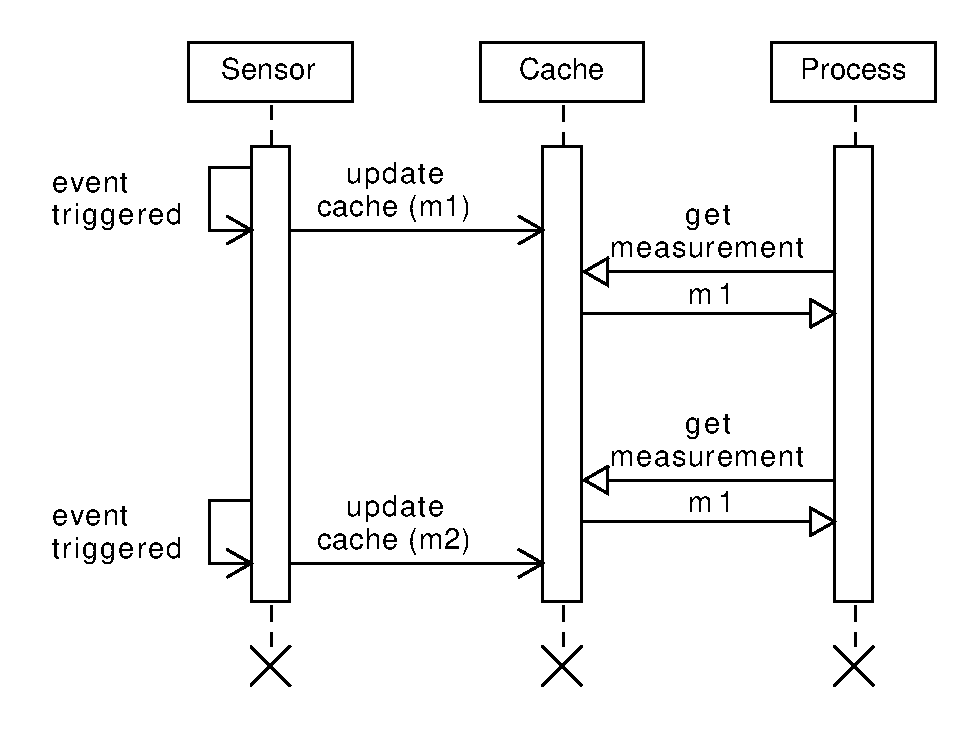
\includegraphics[width=\linewidth]{sensor_providers/cache_example_1}
  \caption{No events between requests.}
  \label{fig:cache_no_event_between}
\end{subfigure}
\begin{subfigure}[!t]{.5\textwidth}
  \centering
  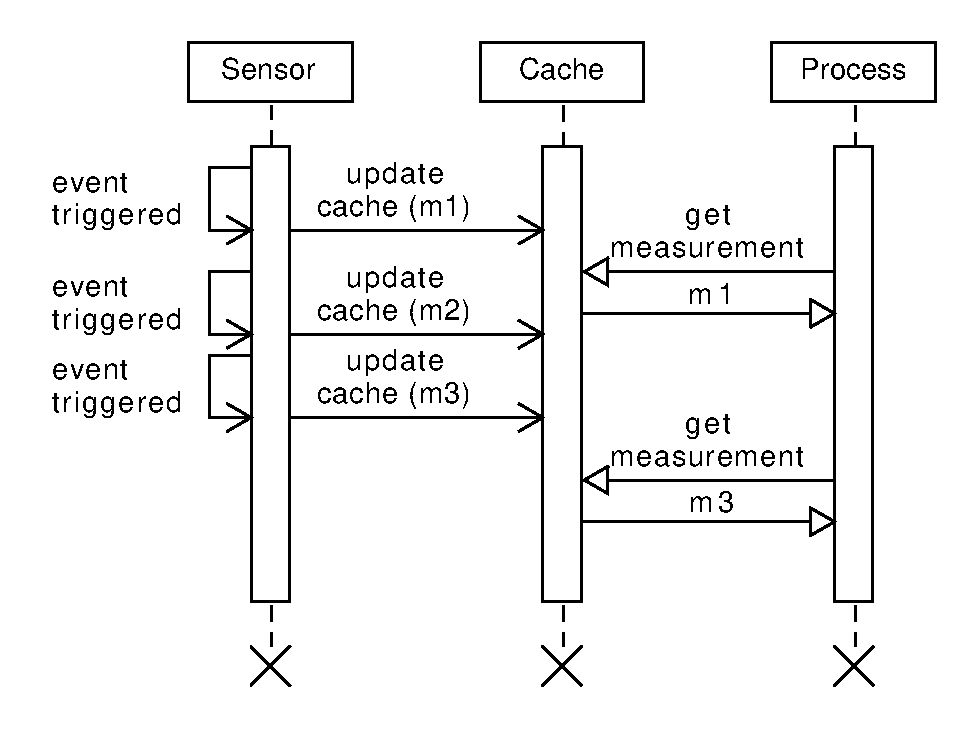
\includegraphics[width=\linewidth]{sensor_providers/cache_example_2}
  \caption{Multiple events between requests.}
  \label{fig:cache_multiple_event_between}
\end{subfigure}
\caption{Measurement caching.}
\label{fig:cache_examples}
\end{figure}
\FloatBarrier

One issue this design might introduce is that we rely on these sensor events being raised eventually. The cache must contain some default value for a sensor, if this is not the case, which could potentially pollute the measurements until the first event is triggered. This means that until the first event is raised other processes will be answered with default values. Other types of data sources, which are not event driven, such as Wi-Fi, are, as mentioned in \secref{sec:deriving_the_context_from_sensors}, available on demand meaning that we are able to acquire the access point data at any given time as long as Wi-Fi is enabled, meaning that some data sources already provide the desired behavior. Some of these on demand sensors might take some time to acquire the information. An example of this could be triangulation based on satellites for GPS. A potential problem here, in regards to timing, is therefore latency before the underlying system is ready to return the data to the caller. This effectively means that the first few measurements for some of the sensors will not reflect the reality they measure, since they have not taken any measurements yet. However, since the default values from sensors are distinguishable from actual measurements, this should not be a problem for customers.

\subsection{Sensor Provider}
\label{sub:providing_sensor_data_implementation}
We have implemented our Sensor Provider as an abstract class called \mono{SensorProvider}, which must be subclassed for each type of available sensor, both for sensors found on the actual Android devices which runs the application, but also for external sensors, such as those found in a Microsoft Band 2. The abstract class provides functionality that makes it easy to implement specialized implementations for every sensor that we have. Sub-classes of the abstract \mono{SensorProider}, must specify a type argument, \mono{MeasurementT}, describing the type of the measurements which the implementation will make. Besides this, the following methods must also be implemented on the specializations:

% The common interface for these sensor providers is implemented by the following methods:

\begin{description}
	\item[\mono{boolean isSensorAvailable()}] should return \mono{true} if the sensor is currently available, and ready to make measurements. Should return \mono{false} if the sensor is unavailable or not present on the device. Overriding this function should be simple for most build-in sensors which are always available if they are included in a device. It should be sufficient with a simple system call, to check if the sensor is present in the device, here. But overriding with function for other data sources such as WiFi, where the physical presence of a WiFi radio in the device does not imply that the radio is turned on and active, might prove more complicated.   

	\item[\mono{SensorType getSensorType()}] should return the \mono{SensorType} that the sensor provider implementation will utilize. For instance \mono{SensorType.BAROMETER}.

	\item[\mono{EventListenerRegistrationManager createRegManager()}] should return an instance of a class that implements the \mono{EventListenerRegistrationManager} interface. This interface will enforce the class to implement the following two methods: \mono{void register(int frequency)} and \mono{void unregister()}. These methods will be used by the \mono{SensorProvider} implementation to register the sensor and thereby acquire some resources, e.g. registering an event listener or start a thread, when the specific sensor is needed, and unregister them, and free the required resources, when they are not.

  \item[\mono{MeasurementT getDefaultMeasurement()}] Should return a default instance of the \mono{MeasurementT} that the subclass is parameterized with, for instance \mono{FloatMeasurement}.
\end{description}

Besides implementing these methods, the specializations must also call the \mono{void onNewMeasurement(MeasurementT)}, which will override the cached value, as described in \figref{fig:cache_examples}. With these measurements registered, the \mono{SensorProvider}, and in effect all of the sub-classes, are now able to construct \mono{Sample} objects by reading measurements from the cache with the specific intervals. 

\subsubsection{Implementing a Sensor Provider}
Because of the abstract \mono{SensorProvider} class, new sensors can be implemented into the system with very few lines of code. An example of such an implementation can be seen in \lstref{lst:sensor_provider_acclerometer}, which shows how the \mono{AccelerometerSensorProvider} implements and uses the methods described above to make measurements from the phones accelerometer available to our application. A developer has to write relative few lines of code to enable such a provider for a any new type of sensor. To do so, the we have, as seen in \lineref{line:sensor_provider_extends}, subclassed \mono{SensorProvider} with the generic parameter \mono{FloatTripleMeasurement} which is the type of measurement the accelerometer produces. Furthermore, we have to override the abstract methods as previously stated: 

\begin{description}
  \item[\mono{boolean isSensorAvailable()}] is overridden in \linesref{line:isSensorAvailable_start}{line:isSensorAvailable_end}. Here we check if the phone has the system feature \mono{FEATURE\_SENSOR\_ACCELEROMETER}; if this is the case, we are able to measure accelerometer.

  \item[\mono{SensorType getSensorType()}] is overridden in \linesref{line:getSensorType_start}{line:getSensorType_end}. This method simply return the enum value \mono{ACCELEROMETER}.

  \item[\mono{EventListenerRegistrationManager createRegManager()}] is overridden in \linesref{line:createRegManager_start}{line:createRegManager_end} and will first construct a listener, registering new measurements whenever the sensor outputs new values. We do not wish to do anything when the accuracy changes, so this block is empty. Lastly we create the registration manager, based on fields found on the \mono{SensorProvider} class, and the listener we created.

  \item[\mono{FloatTripleMeasurement getDefaultMeasurement()}] is overridden in \linesref{line:getDefaultMeasurement_start}{line:getDefaultMeasurement_end}, simply returning a new \mono{FloatTripleMeasuremen} instance with no values provided, causing the values to be initialized to \mono{0.0f}.
\end{description}

\lstinputlisting[
   style = Java,
   caption = {Implementation of sensor provider for Accelerometer.},
   label = {lst:sensor_provider_acclerometer},
   float=!htbp,
]{content/gathering_sensor_data/code_snippets/sensor_provider_acclerometer.java}
\FloatBarrier

\subsection{Gathering Data from the Microsoft Band 2}
Due to the structure of sensor providers, as described in \secref{sub:providing_sensor_data_implementation}, it is relatively easy to implement functionality that will gather information from the Microsoft Band 2 smart band. The only major difference between the Microsoft Band sensors, and the sensors in an android smartphone, is that a connection between the smart band and the phone has to be made. This connection has to be made in all of the band sensor providers; due to this, we implemented an abstract class called \mono{SensorProviderBand}, which implements the method \mono{getConnectedBandClient()} which will try to establish a connection to the smart band, through the required Microsoft Health application. The method can be seen in \lstref{lst:get_connected_band_client}. The method return a boolean, indicating if the connection were established or not. However, currently, we do not do anything specific when the connection fails, and we simply try again at a later point in time. For a more detailed description of how the application communicated through the Microsoft Health application, see \secref{sec:device}.

\lstinputlisting[
   style = Java,
   caption = {Establishing a connection between the phone and the smart band.},
   label = {lst:get_connected_band_client},
   float=!htbp,
]{content/gathering_sensor_data/code_snippets/get_connected_band_client.java}
\FloatBarrier

\subsection{Asynchronous Delivery of Samples}

A \mono{SensorProvider} subclass is, with the the requirements implemented, able to provide a list of \mono{Sample} instances at some point in the future through a call to a member function on the abstract \mono{SensorProvider} class. This is captured by letting the method return an instance of \mono{\mono{Future<List<Sample>>. A \mono{Future} object is a reference to some other object which represents the result of some computation being performed on another thread. A client of \mono{SensorProvider} instances can the request multiple of such \mono{Future} instances and then, once having all the desired \mono{Future} instances, choose to synchronously call a \mono{get()} on the \mono{Future} instances and effectively wait for the asynchronous computations to complete.
\\\\
Using futures and not saving any intermediary state persistently might prove to be a problem for Snapshots which are configured to collect data for longer periods of time as they might quickly fill up the memory because the objects referenced by the \mono{Future} instances is not dereferenced, and thereby freed, before the tasks behind the \mono{Future} instances are completed. Further development on how to minimize memory consumption for Snapshot collection should be pursued.
